%=====================================================================
\section{Survival of wall defects and docking in ovals and ellipses}\label{sec:ssurv}
Same measures as Sec.~\ref{sec:csurv}; the survival figure (Fig.~\ref{fig:surv}) contains all shapes.
\begin{table}[H]\centering\small
\caption{Wall-visit survival and docking, $k=6$ unless noted (seeds: H34 and H48 3, ellipses 2, lobe oval 3).
Escape rate in $10^{-3}$ per wall defect per time unit (mean $\pm$ s.e.\ over seeds); docking rate per 100 cells of wall per time
unit; $P_\mathrm{dock}$: fraction of bulk $+\half$ episodes that end at the wall. Median times in the bulk before docking (21--76 time units) are in \texttt{reports/master/data/survival\_docking.txt}.}\label{tab:ssurv}
\begin{adjustbox}{max width=\textwidth}
\begin{tabular}{lcccccccc}\toprule
cavity & aspect & visits & wall $+\half$ & escape rate & $S(1000)$ & $t_{1/2}$ & dock rate & $P_\mathrm{dock}$\\\midrule
circle $1.43\,\la$ & 1 & 73 & 10.0 & $0.34\pm0.07$ & 0.50 & 1000 & 0.0015 & 0.10\\
circle $2.15\,\la$ & 1 & 98 & 9.9 & $0.41\pm0.16$ & 0.51 & 1044 & 0.0014 & 0.04\\
H34 $b/a=2.5$ & 1.18 & 145 & 9.9 & $0.65\pm0.07$ & 0.39 & 666 & 0.0030 & 0.19\\
H34 $b/a=2.0$ & 1.29 & 668 & 9.1 & $3.2\pm0.2$ & 0.05 & 100 & 0.015 & 0.54\\
H34 $b/a=1.6$ & 1.51 & 1039 & 8.1 & $6.0\pm0.1$ & 0.009 & 84 & 0.024 & 0.67\\
H34 $b/a=1.3$ & 1.94 & 998 & 8.2 & $5.7\pm0.1$ & 0.007 & 98 & 0.024 & 0.73\\
H48 $b/a=2.5$ & 1.18 & 577 & 9.2 & $2.7\pm0.1$ & 0.07 & 102 & 0.009 & 0.27\\
H48 $b/a=2.0$ & 1.29 & 1433 & 6.2 & $10.8\pm0.5$ & 0.001 & 52 & 0.022 & 0.46\\
H48 $b/a=1.6$ & 1.51 & 1350 & 6.2 & $10.6\pm0.5$ & 0 & 62 & 0.022 & 0.47\\
H48 $b/a=1.3$ & 1.94 & 1372 & 6.2 & $10.5\pm0.5$ & 0 & 62 & 0.023 & 0.53\\
ellipse $\varepsilon=1.2$ & 1.2 & 120 & 9.9 & $0.83\pm0.03$ & 0.33 & 368 & 0.0042 & 0.30\\
ellipse $\varepsilon=1.5$ & 1.5 & 731 & 7.9 & $6.4\pm0.05$ & 0.009 & 90 & 0.025 & 0.67\\
ellipse $\varepsilon=2.0$ & 2.0 & 788 & 7.4 & $7.2\pm0.1$ & 0.003 & 72 & 0.025 & 0.72\\
lobe oval ($k=3$) & 1.38 & 530 & 2.8 & $8.3\pm0.3$ & 0.002 & 70 & 0.013 & 0.61\\\bottomrule
\end{tabular}
\end{adjustbox}
\end{table}
\begin{figure}[H]\centering
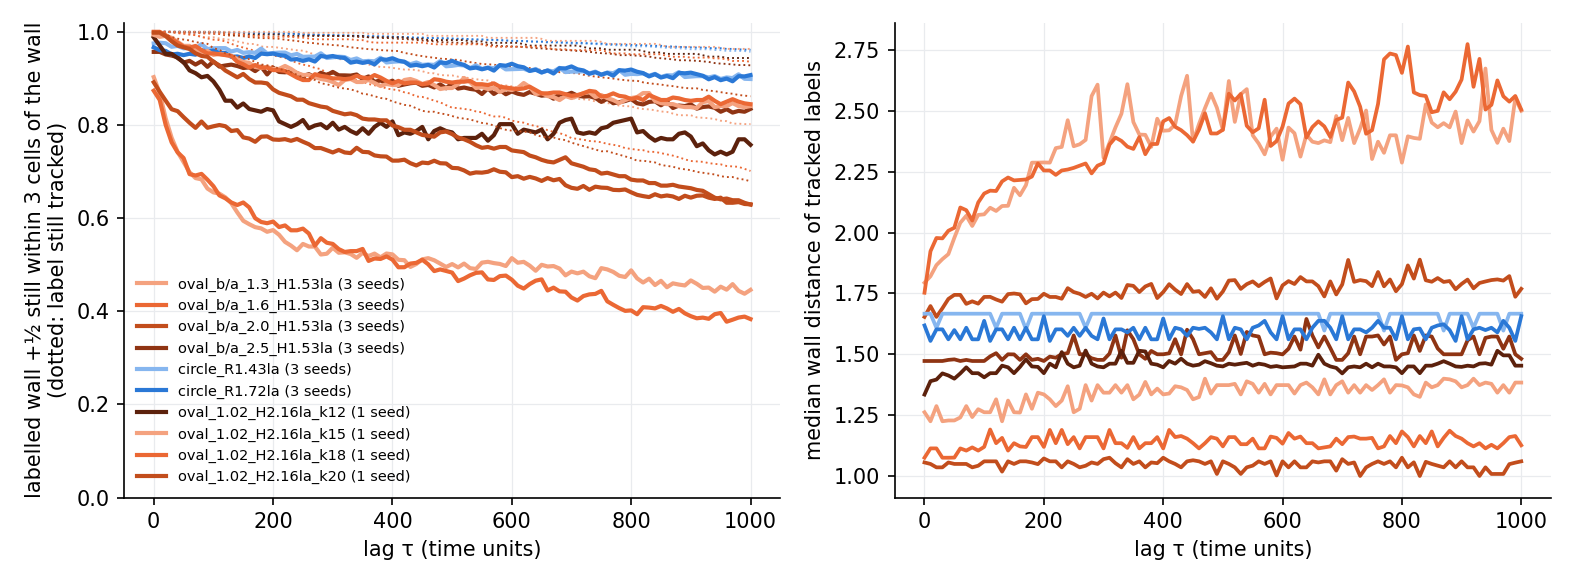
\includegraphics[width=\textwidth]{labels_small_ovals.png}
\caption{Label survival: small ovals ($b/a=2.5\to1.3$, 3 seeds, orange light to dark), circles of $1.43$ and $1.72\,\la$ (blue, 3 seeds) and the pinched oval at $k=12$--20 (1 seed). Left: fraction of labelled wall defects within 3 cells of the wall (dotted: label still tracked); right: median wall distance of tracked labels.}\label{fig:labsmall}
\end{figure}
\begin{figure}[H]\centering
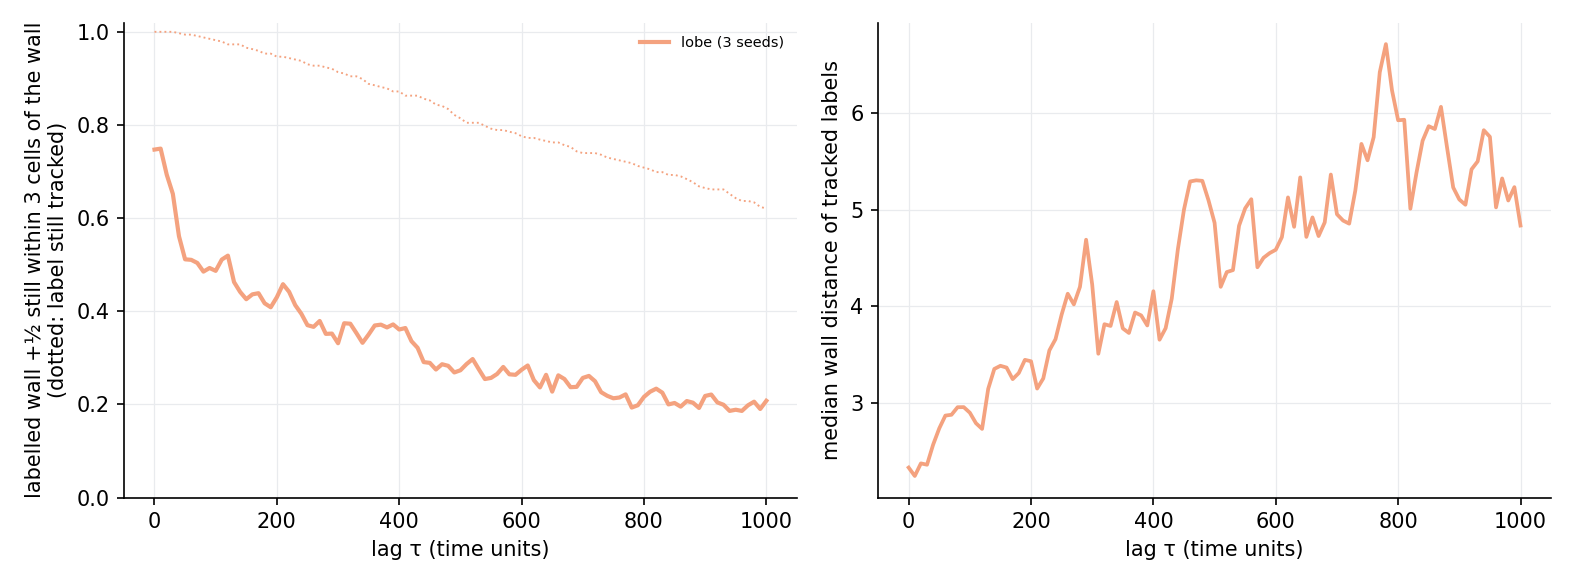
\includegraphics[width=0.85\textwidth]{labels_lobe_oval.png}
\caption{Label survival in the lobe-shaped oval ($k=3$, seed 1 shown; seeds 2--3: 16--28\% at the wall after 1000).}\label{fig:lablobe}
\end{figure}
\begin{itemize}
  \item \textbf{Wall defects in elongated cavities do not stay:} escape rates $6$--$11\times10^{-3}$, 17--30$\times$ the clean circles; half
        of the wall visits end within 50--100 time units, and essentially none last 1000 (circles: half last longer than 1000). Label
        survival agrees: in the small ovals 37--50\% of labels at the wall after 1000 for $b/a\le1.6$ (circle 87--94\%), in the larger ovals
        6--39\%.
  \item \textbf{Docking becomes the norm:} 46--73\% of bulk $+\half$ excursions end at the wall in elongated cavities, against 4--10\% in
        clean circles. The layer and the bulk exchange continuously, so ``layer'' and ``bulk'' stop being separate populations.
  \item \textbf{The crossover is the same as for the charge, pinning and the vortex:} round shapes ($b/a=2.5$, $\varepsilon=1.2$) stay close
        to circles (escape 0.65--0.83$\times10^{-3}$ at half-length $1.53\,\la$), elongated ones (aspect $\ge1.5$) are fully exchanging;
        $b/a=2.0$ (aspect 1.29) is intermediate.
  \item \textbf{Size matters on top of shape:} at half-length $2.16\,\la$ even $b/a=2.5$ escapes 4$\times$ faster than at $1.53\,\la$, and the
        elongated shapes saturate at $\approx10^{-2}$ with only 6 of 10 sites occupied; at this size circles are still clean.
  \item At most 10\% of wall visits end in annihilation: the layer empties by undocking, not by annihilation of wall defects.
\end{itemize}
